\documentclass[unknownkeysallowed]{beamer}
\usepackage[french,english]{babel}
\usepackage{./tex/sty/beamer_js}
\usepackage{./tex/sty/shortcuts_js}
\usepackage{biblatex}
\addbibresource{./biblio/references.bib}
\newcommand{\trans}[1]{{#1}^\intercal} % transposition
\usepackage{csquotes}

\begin{document}


%%%%%%%%%%%%%%%%%%%%%%%%%%%%%%%%%%%%%%%%%%%%%%%%%%%%%%%%%%%%%%%%%%%%%%%%%%%%%%%
%%%%%%%%%%%%%%%%%%%%%%             Headers               %%%%%%%%%%%%%%%%%%%%%%
%%%%%%%%%%%%%%%%%%%%%%%%%%%%%%%%%%%%%%%%%%%%%%%%%%%%%%%%%%%%%%%%%%%%%%%%%%%%%%%



%%%%%%%%%%%%%%%%%%%%%%%%%%%%%%%%%%%%%%%%%%%%%%%%%%%%%%%%%%%%%%%%%%%%%%%%%%%%%%%
\begin{frame}
\bigskip
\bigskip
\begin{center}{
\LARGE\color{marron}
\textbf{HMMA 308 : Machine Learning}}
\vspace{0.5cm}


\color{marron}
\textbf{Lasso vs FoBa}
\end{center}

\vspace{0.5cm}

\begin{center}
\textbf{Ophélie Coiffier} \\
\vspace{0.1cm}
\url{https://github.com/opheliecoiffier/LASSOvsFoBa}\\
\vspace{0.5cm}
Université de Montpellier \\
\end{center}

\centering
\includegraphics[width=0.13\textwidth]{./images/Logo.pdf}

\end{frame}
%%%%%%%%%%%%%%%%%%%%%%%%%%%%%%%%%%%%%%%%%%%%%%%%%%%%%%%%%%%%%%%%%%%%%%%%%%%%%%%



%%%%%%%%%%%%%%%%%%%%%%%%%%%%%%%%%%%%%%%%%%%%%%%%%%%%%%%%%%%%%%%%%%%%%%%%%%%%%%%
%%%%%%%%%%%%%%%%%%%%%%%%       PLAN      %%%%%%%%%%%%%%%%%%%%%%%%%%%%%%%%%%%%%%
%%%%%%%%%%%%%%%%%%%%%%%%%%%%%%%%%%%%%%%%%%%%%%%%%%%%%%%%%%%%%%%%%%%%%%%%%%%%%%%



%%%%%%%%%%%%%%%%%%%%%%%%%%%%%%%%%%%%%%%%%%%%%%%%%%%%%%%%%%%%%%%%%%%%%%%%%%%%%%%
\begin{frame}{Table of Contents}
\tableofcontents[hideallsubsections]
\end{frame}
%%%%%%%%%%%%%%%%%%%%%%%%%%%%%%%%%%%%%%%%%%%%%%%%%%%%%%%%%%%%%%%%%%%%%%%%%%%%%%%



%%%%%%%%%%%%%%%%%%%%%%%%%%%%%%%%%%%%%%%%%%%%%%%%%%%%%%%%%%%%%%%%%%%%%%%%%%%%%%%
\AtBeginSection[]
{
\begin{frame}<beamer>{Table of Contents}
\tableofcontents[currentsubsection,
    hideothersubsections,
    sectionstyle=show/shaded,
]
\end{frame}
}
%%%%%%%%%%%%%%%%%%%%%%%%%%%%%%%%%%%%%%%%%%%%%%%%%%%%%%%%%%%%%%%%%%%%%%%%%%%%%%%




%%%%%%%%%%%%%%%%%%%%%%%%%%%%%%%%%%%%%%%%%%%%%%%%%%%%%%%%%%%%%%%%%%%%%%%%%%%%%%%
%%%%%%%%%%%%%%%%%%%%%%%%%%%%%%%%%%%%%%%%%%%%%%%%%%%%%%%%%%%%%%%%%%%%%%%%%%%%%%%
\section{Mathematics approach}
\label{sec:Mathematics approach}
%%%%%%%%%%%%%%%%%%%%%%%%%%%%%%%%%%%%%%%%%%%%%%%%%%%%%%%%%%%%%%%%%%%%%%%%%%%%%%
%%%%%%%%%%%%%%%%%%%%%%%%%%%%%%%%%%%%%%%%%%%%%%%%%%%%%%%%%%%%%%%%%%%%%%%%%%%%%%%

%%%%%%%%%%%%%%%%%%%%%%%%%%%%%%%%%%%%%%%%%%%%%%%%%%%%%%%%%%%%%%%%%%%%%%%%%%%%%%%
\subsection*{Introduction}
\label{sub:Intro}
\begin{frame}{Introduction}
To measure the quality of prediction, we use linear prediction model :
\[f(x)=\trans{\beta}x\]
With \[\hat{\beta}=\underset{\beta \in \bbR^d}\argmin\sum_{i=1}^n \Phi(\trans{\beta}x_i, y_i)+\lambda g(\beta)\]
\end{frame}



%%%%%%%%%%%%%%%%%%%%%%%%%%%%%%%%%%%%%%%%%%%%%%%%%%%%%%%%%%%%%%%%%%%%%%%%%%%%%%%
\subsection{The Lasso method}
\label{sub:Lasso}
%%%%%%%%%%%%%%%%%%%%%%%%%%%%%%%%%%%%%%%%%%%%%%%%%%%%%%%%%%%%%%%%%%%%%%%%%%%%%%%

%%%%%%%%%%%%%%%%%%%%%%%%%%%%%%%%%%%%%%%%%%%%%%%%%%%%%%%%%%%%%%%%%%%%%%%%%%%%%%%
\begin{frame}{The Lasso method}
\vspace{0.4cm}
Method uses $L_1$ regularization.\\
We have \[\hat{\beta}=\underset{\beta \in \bbR^d}\argmin\sum_{i=1}^n \Phi(\trans{\beta}x_i, y_i)+\lambda ||\beta||_1\]
$2$ issues :
\begin{itemize}
    \item strong assumptions
    \item large regularization parameter ($\lambda$)
\end{itemize}
\end{frame}
%%%%%%%%%%%%%%%%%%%%%%%%%%%%%%%%%%%%%%%%%%%%%%%%%%%%%%%%%%%%%%%%%%%%%%%%%%%%%%%


%%%%%%%%%%%%%%%%%%%%%%%%%%%%%%%%%%%%%%%%%%%%%%%%%%%%%%%%%%%%%%%%%%%%%%%%%%%%%%%
\subsection{The OMP method}
\label{sub:OMP}
%%%%%%%%%%%%%%%%%%%%%%%%%%%%%%%%%%%%%%%%%%%%%%%%%%%%%%%%%%%%%%%%%%%%%%%%%%%%%%%



%%%%%%%%%%%%%%%%%%%%%%%%%%%%%%%%%%%%%%%%%%%%%%%%%%%%%%%%%%%%%%%%%%%%%%%%%%%%%%%
\begin{frame}{The OMP method}
\vspace{1cm}
    "Orthogonal Match Pursuit" : forward greedy algorithm
\vspace{1cm}
\newline
	\only<2->{\textbf{Principle :} Add feature at every step to reduce the squared error $\&$ Calculate its error} \newline
	\visible<3->{\textbf{Ability :} Select relevant features} \newline
	\only<4->{\textbf{Main issue :} Never correct mistakes made earlier steps} \newline
	\visible<5->{\textbf{Solution :} Backward greedy algorithm ?} \newline
\end{frame}

%%%%%%%%%%%%%%%%%%%%%%%%%%%%%%%%%%%%%%%%%%%%%%%%%%%%%%%%%%%%%%%%%%%%%%%%%%%%%%%

%%%%%%%%%%%%%%%%%%%%%%%%%%%%%%%%%%%%%%%%%%%%%%%%%%%%%%%%%%%%%%%%%%%%%%%%%%%%%%%
\subsection{The FoBa algorithm (Lars method)}
\label{sub:FoBa}
%%%%%%%%%%%%%%%%%%%%%%%%%%%%%%%%%%%%%%%%%%%%%%%%%%%%%%%%%%%%%%%%%%%%%%%%%%%%%%%

%%%%%%%%%%%%%%%%%%%%%%%%%%%%%%%%%%%%%%%%%%%%%%%%%%%%%%%%%%%%%%%%%%%%%%%%%%%%%%%
\begin{frame}{The FoBa algorithm (Lars method)}
"Forward-Backward" greedy algorithm
\vspace{1cm}
\newline
    \textbf{Principle :}
    \newline
	\only<2->{1) Use Forward greedy step} \newline
	\visible<3->{2) Until squared error increase is no more than half of the squared error decrease in the earlier forward step} \newline
	\only<4->{3) Use Backward greedy step $\&$ adaptive Backward step} \newline
	\visible<5->{*) \textbf{Adaptive backward function :}
	\begin{itemize}
	\item Make sure that we progress
	\end{itemize}
	}
\end{frame}

%%%%%%%%%%%%%%%%%%%%%%%%%%%%%%%%%%%%%%%%%%%%%%%%%%%%%%%%%%%%%%%%%%%%%%%%%%%%%%%

%%%%%%%%%%%%%%%%%%%%%%%%%%%%%%%%%%%%%%%%%%%%%%%%%%%%%%%%%%%%%%%%%%%%%%%%%%%%%%%
\subsection*{Comparison between Lasso and FoBa}
%%%%%%%%%%%%%%%%%%%%%%%%%%%%%%%%%%%%%%%%%%%%%%%%%%%%%%%%%%%%%%%%%%%%%%%%%%%%%%%

%%%%%%%%%%%%%%%%%%%%%%%%%%%%%%%%%%%%%%%%%%%%%%%%%%%%%%%%%%%%%%%%%%%%%%%%%%%%%%%
\begin{frame}{Comparison between Lasso and FoBa}

\begin{table}
        \centering
        \begin{tabular}{| c | c |}
        \hline
        \begin{bf} Similarity \end{bf} &
        \begin{bf} Difference \end{bf} \\
        \hline
        Path-following algorithm &  Conditions to find threshold \\
        Large regularization parameter & Bias \\
        Mistakes in earlier step &  \\
        \hline
        \end{tabular}
    \end{table}
\end{frame}

%%%%%%%%%%%%%%%%%%%%%%%%%%%%%%%%%%%%%%%%%%%%%%%%%%%%%%%%%%%%%%%%%%%%%%%%%%%%%%%


%%%%%%%%%%%%%%%%%%%%%%%%%%%%%%%%%%%%%%%%%%%%%%%%%%%%%%%%%%%%%%%%%%%%%%%%%%%%%%%
\section{Examples}
\label{sec:example}
%%%%%%%%%%%%%%%%%%%%%%%%%%%%%%%%%%%%%%%%%%%%%%%%%%%%%%%%%%%%%%%%%%%%%%%%%%%%%%%
%%%%%%%%%%%%%%%%%%%%%%%%%%%%%%%%%%%%%%%%%%%%%%%%%%%%%%%%%%%%%%%%%%%%%%%%%%%%%%%

%%%%%%%%%%%%%%%%%%%%%%%%%%%%%%%%%%%%%%%%%%%%%%%%%%%%%%%%%%%%%%%%%%%%%%%%%%%%%%
\begin{frame}{Introduction}
Loss function used : \[MSE = \frac{1}{n} \sum_{i=1}^n (\hat{Y}_i-Y_i)^2\]

\textbf{Principle : }
\begin{itemize}
    \item Randomly partition into $50$ training points and \textit{nb} test points
    \item Predict variable
    \item Compare MSE for each methods and for each groups
\end{itemize}
\end{frame}
%%%%%%%%%%%%%%%%%%%%%%%%%%%%%%%%%%%%%%%%%%%%%%%%%%%%%%%%%%%%%%%%%%%%%%%%%%%%%%



%%%%%%%%%%%%%%%%%%%%%%%%%%%%%%%%%%%%%%%%%%%%%%%%%%%%%%%%%%%%%%%%%%%%%%%%%%%%%%%
\subsection{\textit{Boston Housing} data}
\label{sub:Boston Housing data}
%%%%%%%%%%%%%%%%%%%%%%%%%%%%%%%%%%%%%%%%%%%%%%%%%%%%%%%%%%%%%%%%%%%%%%%%%%%%%%%

%%%%%%%%%%%%%%%%%%%%%%%%%%%%%%%%%%%%%%%%%%%%%%%%%%%%%%%%%%%%%%%%%%%%%%%%%%%%%%%
\begin{frame}{\textit{Boston Housing} data}
\textbf{Data : }$506$ census tracts from $1970$ census\\
\hspace{1.2cm}       $14$ features\\
\vspace{0.5cm}
\textbf{Y : }housing price\\
\vspace{0.5cm}
\textbf{Principle : }$50$ training points / $456$ test points\\
We repeat $50$ times MSE calculations and compare MSE obtained\\
With a sparsity between $1$ and $10$.
\end{frame}
%%%%%%%%%%%%%%%%%%%%%%%%%%%%%%%%%%%%%%%%%%%%%%%%%%%%%%%%%%%%%%%%%%%%%%%%%%%%%%%

%%%%%%%%%%%%%%%%%%%%%%%%%%%%%%%%%%%%%%%%%%%%%%%%%%%%%%%%%%%%%%%%%%%%%%%%%%%%%%%
\begin{frame}{\textit{Boston Housing} data}
\begin{figure}
    \centering
    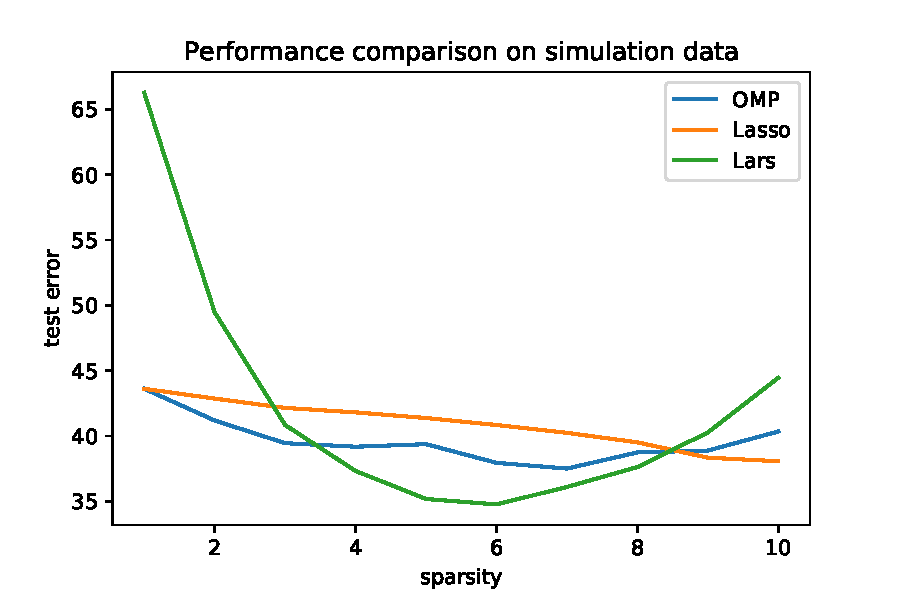
\includegraphics[scale=0.35]{./images/test_error_housing.pdf}
    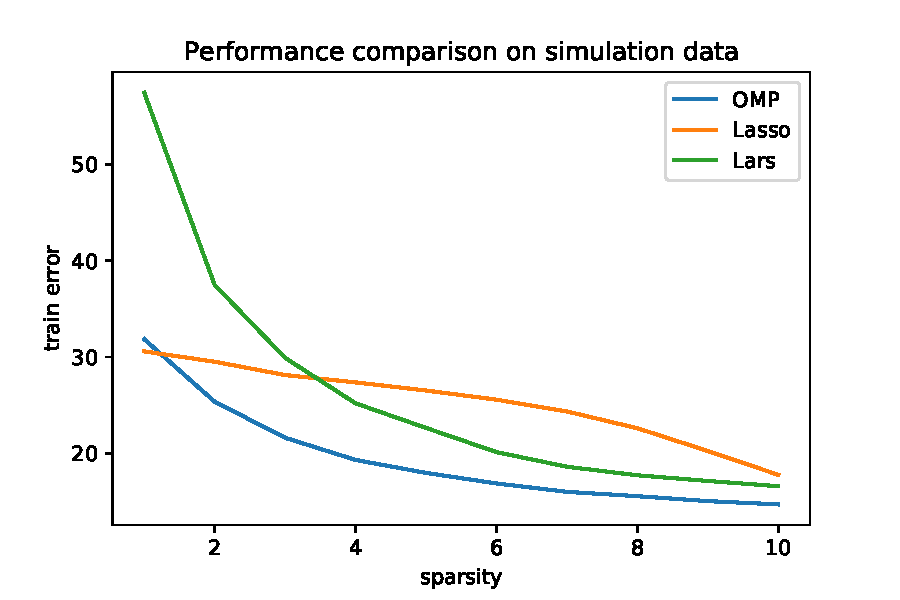
\includegraphics[scale=0.35]{./images/training_error_housing.pdf}
    \caption{MSE depending on sparsity for the $3$ methods and for the $2$ groups.}
\end{figure}
\end{frame}
%%%%%%%%%%%%%%%%%%%%%%%%%%%%%%%%%%%%%%%%%%%%%%%%%%%%%%%%%%%%%%%%%%%%%%%%%%%%%%%

%%%%%%%%%%%%%%%%%%%%%%%%%%%%%%%%%%%%%%%%%%%%%%%%%%%%%%%%%%%%%%%%%%%%%%%%%%%%%%%
%%%%%%%%%%%%%%%%%%%%%%%%%%%%%%%%%%%%%%%%%%%%%%%%%%%%%%%%%%%%%%%%%%%%%%%%%%%%%%%
\subsection{\textit{Ionosphere} data}
\label{sub:Ionosphere data}
%%%%%%%%%%%%%%%%%%%%%%%%%%%%%%%%%%%%%%%%%%%%%%%%%%%%%%%%%%%%%%%%%%%%%%%%%%%%%%%
%%%%%%%%%%%%%%%%%%%%%%%%%%%%%%%%%%%%%%%%%%%%%%%%%%%%%%%%%%%%%%%%%%%%%%%%%%%%%%%

%%%%%%%%%%%%%%%%%%%%%%%%%%%%%%%%%%%%%%%%%%%%%%%%%%%%%%%%%%%%%%%%%%%%%%%%%%%%%%%
\begin{frame}{\textit{Ionosphere} data}
\textbf{Data : }$351$ data points\\
\hspace{1.2cm}  $35$ features\\
\vspace{0.5cm}
\textbf{Y : }binary variable (Y$\in \{0,1\}$)\\
\vspace{0.5cm}
\textbf{Principle : }$50$ training points / $301$ test points\\
We repeat $50$ times MSE calculations and compare MSE obtained\\
With a sparsity between $1$ and $10$.
\end{frame}
%%%%%%%%%%%%%%%%%%%%%%%%%%%%%%%%%%%%%%%%%%%%%%%%%%%%%%%%%%%%%%%%%%%%%%%%%%%%%%%

%%%%%%%%%%%%%%%%%%%%%%%%%%%%%%%%%%%%%%%%%%%%%%%%%%%%%%%%%%%%%%%%%%%%%%%%%%%%%%%
\begin{frame}{\textit{Ionosphere} data}
\begin{figure}
    \centering
    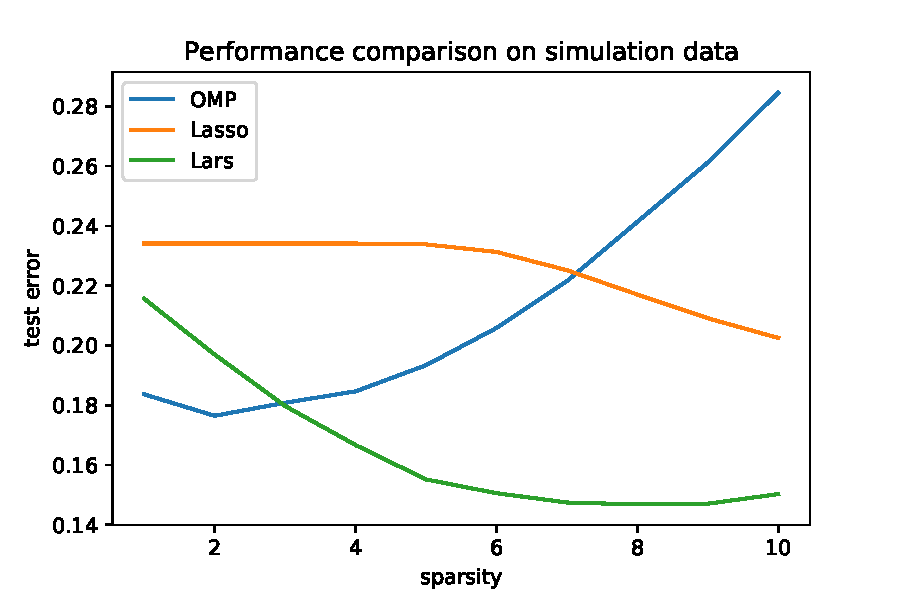
\includegraphics[scale=0.35]{./images/test_error_ionosphere.pdf}
    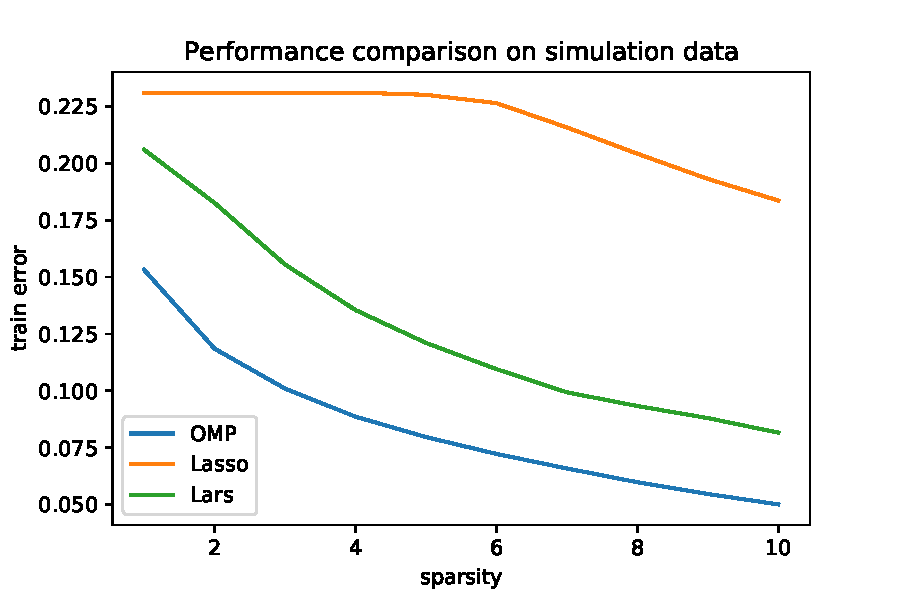
\includegraphics[scale=0.35]{./images/training_error_ionosphere.pdf}
    \caption{MSE depending on sparsity for the $3$ methods and for the $2$ groups.}
\end{figure}
\end{frame}
%%%%%%%%%%%%%%%%%%%%%%%%%%%%%%%%%%%%%%%%%%%%%%%%%%%%%%%%%%%%%%%%%%%%%%%%%%%%%%%


%%%%%%%%%%%%%%%%%%%%%%%%%%%%%%%%%%%%%%%%%%%%%%%%%%%%%%%%%%%%%%%%%%%%%%%%%%%%%%%%
\begin{frame}{Issues}

\begin{itemize}
    \item Representation of Lasso
    \begin{figure}
        \centering
        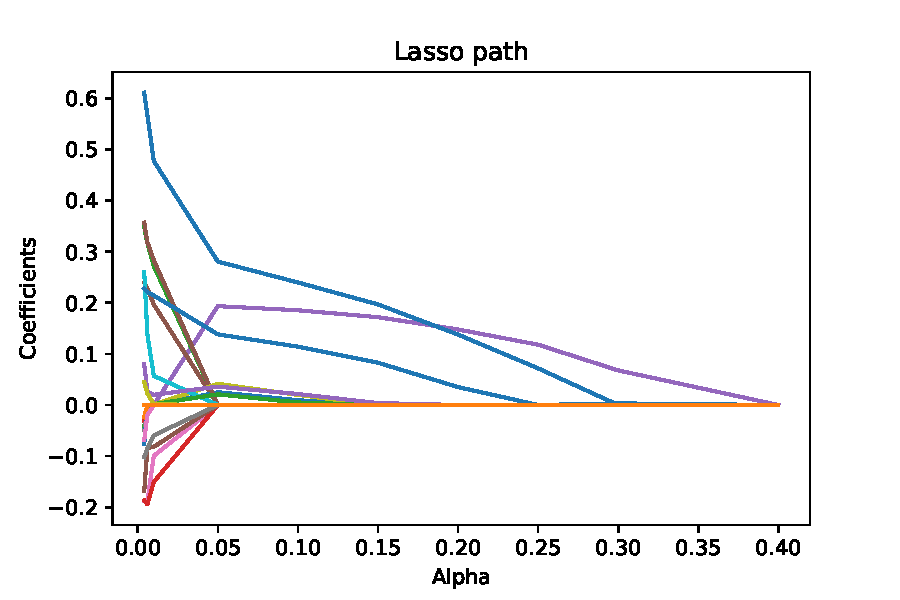
\includegraphics[scale=0.35]{./images/alpha_choice_lasso}
        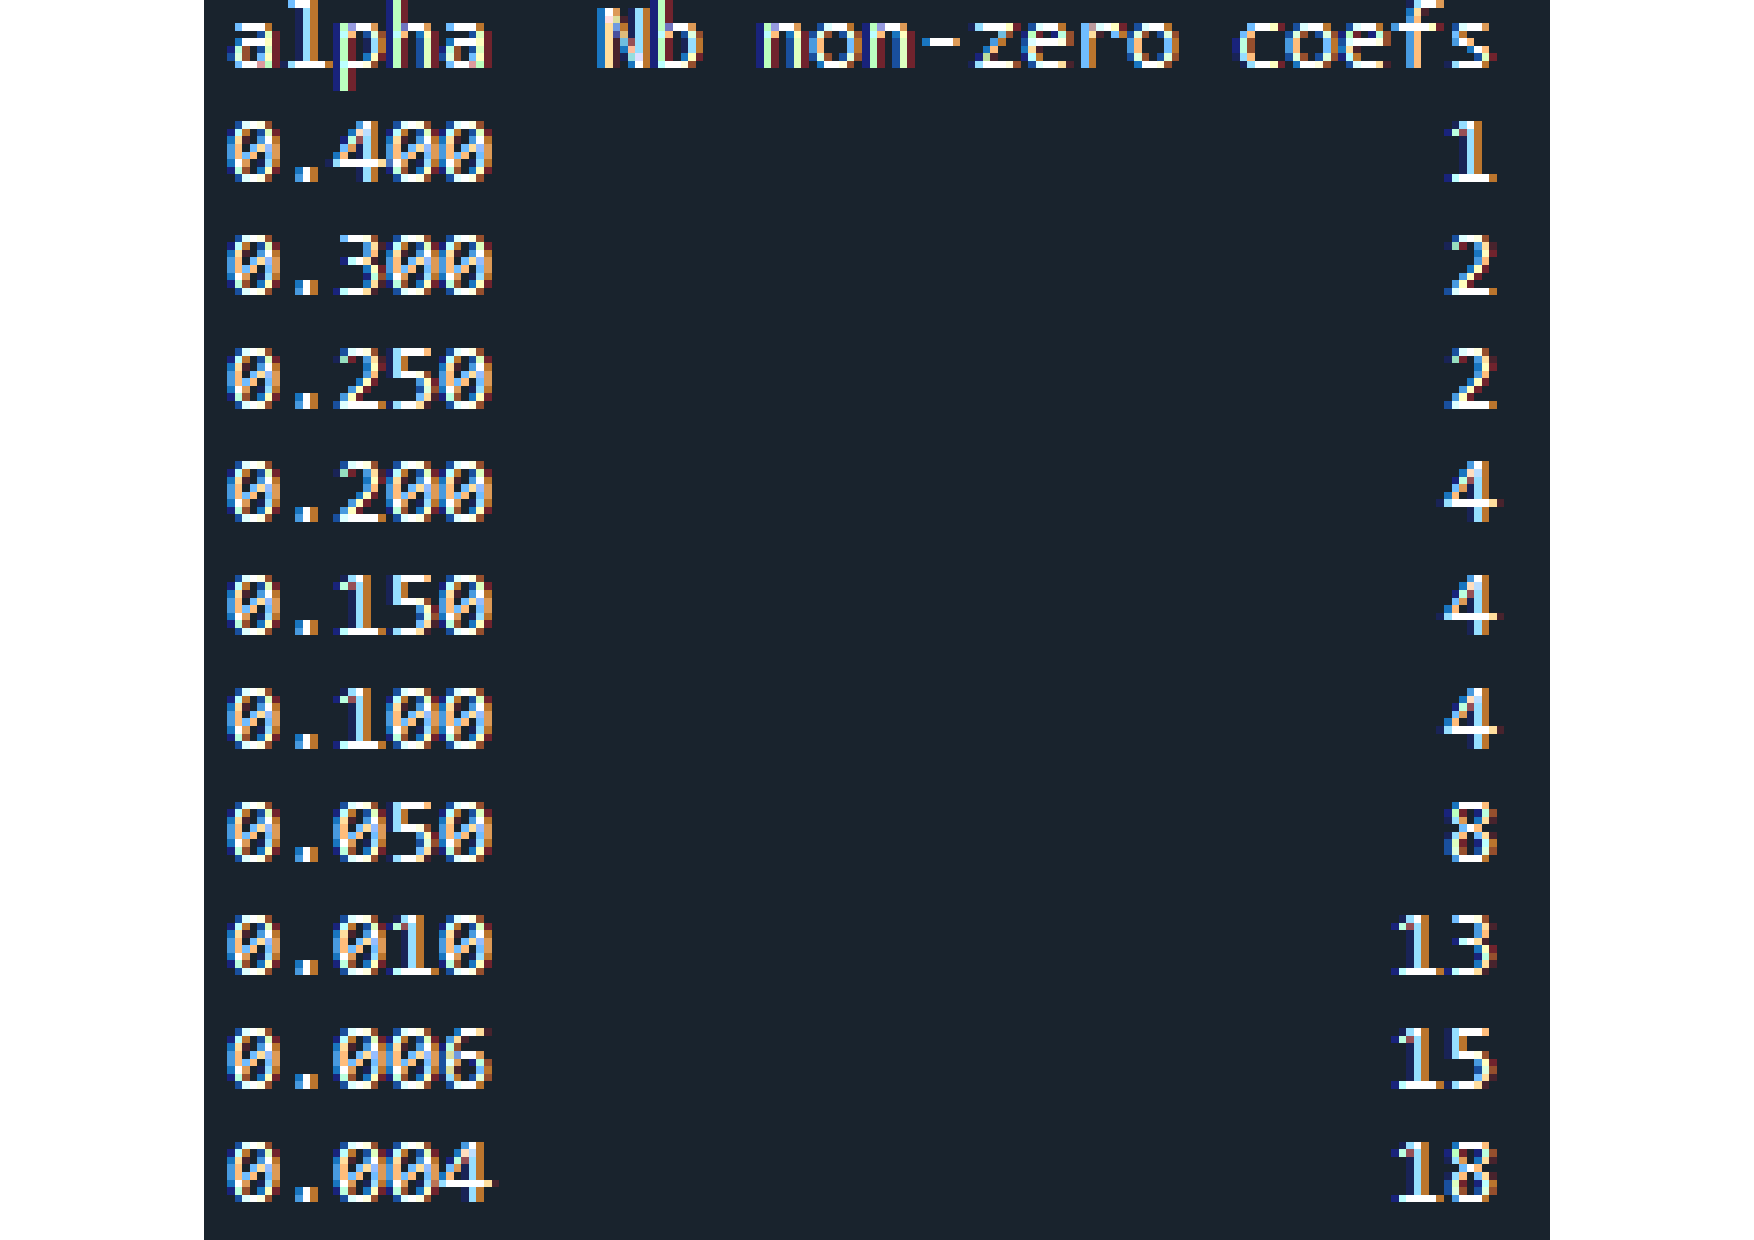
\includegraphics[scale=0.15]{./images/nb_non_zero_ionosphere}
        \caption{Lasso path and non-zero coefficients for Ionosphere data}
    \end{figure}
    \item Differences between our algorithms and these in the article
\end{itemize}
\end{frame}
%%%%%%%%%%%%%%%%%%%%%%%%%%%%%%%%%%%%%%%%%%%%%%%%%%%%%%%%%%%%%%%%%%%%%%%%%%%%%%%


%%%%%%%%%%%%%%%%%%%%%%%%%%%%%%%%%%%%%%%%%%%%%%%%%%%%%%%%%%%%%%%%%%%%%%%%%%%%%%%
%%%%%%%%%%%%%%%%%%%%%%%%%%%%%%%%%%%%%%%%%%%%%%%%%%%%%%%%%%%%%%%%%%%%%%%%%%%%%%%
\section{Conclusion}
\label{sec:conclusion}
%%%%%%%%%%%%%%%%%%%%%%%%%%%%%%%%%%%%%%%%%%%%%%%%%%%%%%%%%%%%%%%%%%%%%%%%%%%%%%%
%%%%%%%%%%%%%%%%%%%%%%%%%%%%%%%%%%%%%%%%%%%%%%%%%%%%%%%%%%%%%%%%%%%%%%%%%%%%%%%


%%%%%%%%%%%%%%%%%%%%%%%%%%%%%%%%%%%%%%%%%%%%%%%%%%%%%%%%%%%%%%%%%%%%%%%%%%%%%%%%
\begin{frame}{Conclusion}

\vspace{0.5cm}
We find these results :
\begin{itemize}
    \item \textbf{Test points :} FoBa for \textit{Ionosphere} data $\&$ FoBa/OMP for \textit{Boston Housing} data
    \item \textbf{Training points :} OMP (depending on sparcity for \textit{Ionosphere} data
\end{itemize}
\vspace{0.2cm}
The article finds :
\begin{itemize}
    \item \textbf{Test points :} FoBa for small sparsity and for \textit{Boston housing} data $\&$ Lasso for \textit{Ionosphere} data
    \item \textbf{Training points :} the mixed algorithm (FoBa)
\end{itemize}
\vspace{0.5cm}
Finally, we must choose the best algorithm and the best method depending on data, sparsity and mathematics conditions that we can check.

\end{frame}

%%%%%%%%%%%%%%%%%%%%%%%%%%%%%%%%%%%%%%%%%%%%%%%%%%%%%%%%%%%%%%%%%%%%%%%%%%%%%%%
\begin{frame}{Bibliography}
\nocite{*}
\printbibliography
\end{frame}
 %%%%%%%%%%%%%%%%%%%%%%%%%%%%%%%%%%%%%%%%%%%%%%%%%%%%%%%%%%%%%%%%%%%%%%%%%%%%%%

\end{document}